


\clearpage
%\counterwithin{figure}{chapter}

%\useunder{\uline}{\ul}{}


%addcontentsline{toc}{chapter}{CAPÍTULO II. Contexto del proyecto \hfill 20}{}

%\addtocontents{toc}{\protect\contentsline{section}{Introducción \hfill 34}{}}
\addtocontents{toc}{\protect\contentsline{chapter}{CAPÍTULO II. Contexto del proyecto \hfill 20}{}{}}




\begin{titlepage}
	
	
	\centering
	\begin{tikzpicture}%opacity=0.5
		\node[inner sep=0pt, ] (image) at (0,0) {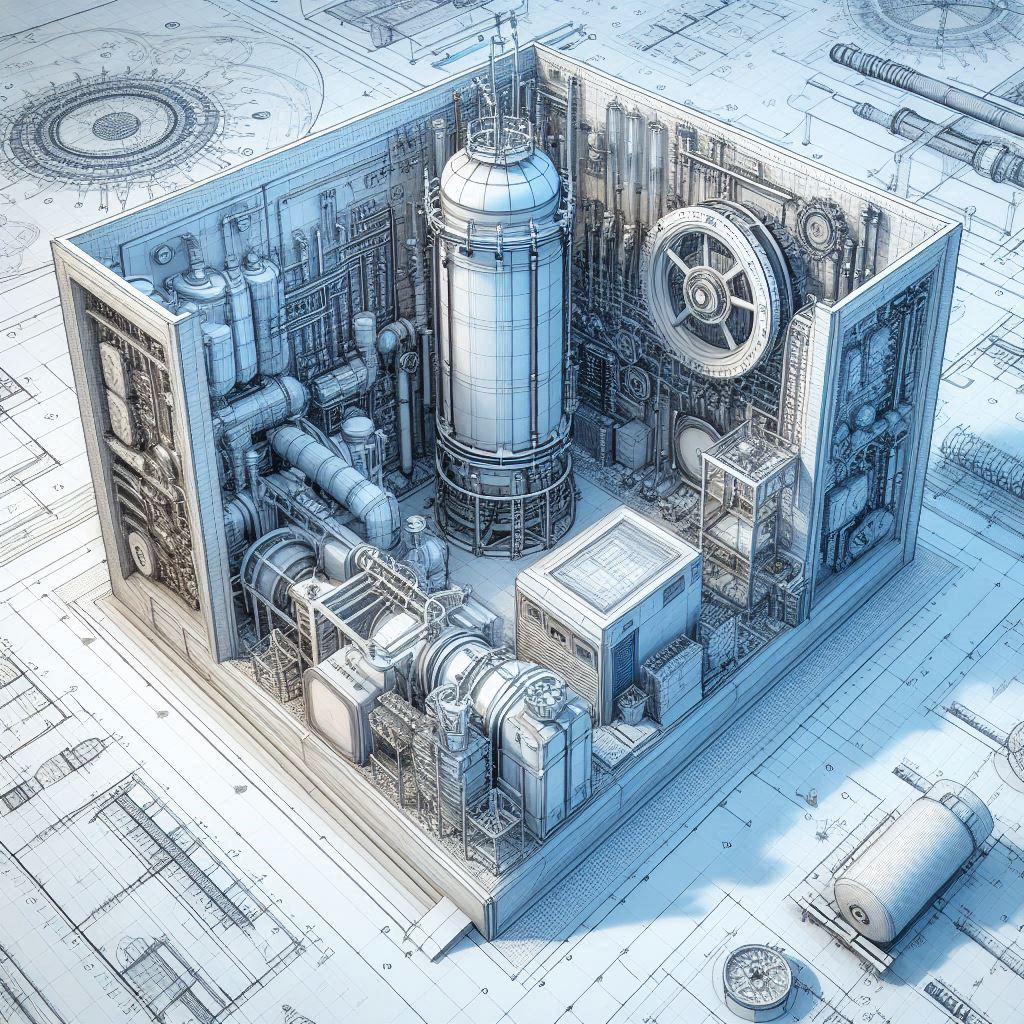
\includegraphics[width=\textwidth]{figures/bg-cap2}};
		\fill [white,path fading=south] (-6,-4) rectangle (6,4);
		\node[black,font=\Huge\bfseries] at (0,3) {Capítulo II};
		\node[black,font=\Huge\bfseries] at (0,2) {Contexto del proyecto};		
		\node[black,font=\LARGE\bfseries] at (0,0.8) {\textit{Estudio del estado de}};
		\node[black,font=\LARGE\bfseries] at (0,-0.2) {\textit{la técnica del proyecto}};
	\end{tikzpicture}
\end{titlepage}




\newpage 

\section*{Introducción}
\addcontentsline{toc}{section}{{Introducción}}\rsp
\setcounter{chapter}{2}
\setcounter{section}{0}
\setcounter{figure}{0}

\setcounter{page}{21}

Es momento de abordar los diferentes contextos en los que nuestro proyecto se ve involucrado, dado que, como se ha manifestado en el capítulo anterior la insulina es un medicamento vital para millones de personas en todo el mundo que viven con diabetes.

Y en específico para habitantes en la zona centro del país, garantizar el almacenamiento seguro y eficaz de la insulina es fundamental para su salud y calidad de vida. Por lo tanto, el diseño de una cámara de refrigeración para la insulina tiene un impacto directo en la salud y bienestar de la población.

Se ha considerado que los avances tecnológicos en refrigeración, como sistemas de control de temperatura precisos y monitoreo remoto, pueden mejorar la eficiencia y confiabilidad de la cámara de refrigeración. Además, consideraremos la integración de tecnologías de seguimiento pueden proporcionar datos importantes sobre el almacenamiento y uso de la insulina.

Así mismo se recapacitado seriamente en el cumplir con las regulaciones y normativas relacionadas con el almacenamiento de medicamentos ya que es fundamental para garantizar la seguridad y eficacia de la insulina. Las cámaras de refrigeración deben cumplir con estándares específicos de la industria farmacéutica y de salud, así como con requisitos de seguridad y calidad establecidos por organismos reguladores.

Últimamente, comprender las características específicas de la insulina, como su sensibilidad a la temperatura y la luz, es esencial para el diseño de la cámara de refrigeración. Las condiciones de almacenamiento inadecuadas pueden comprometer la estabilidad y eficacia de la insulina, lo que podría tener graves consecuencias para los pacientes.






\newpage

\section{Contexto tecnológico}

Desde 2013, la industria del almacenamiento en cadenas de frío\footnote{La cadena de frío es un término aplicado a la manipulación y distribución de alimentos donde el producto se mantiene en condiciones de temperatura adecuadas desde la cosecha, pasando por el proceso de enfriamiento o congelación hasta el punto de venta \cite{Hundy1984}.}   ha crecido a un ritmo impresionante. El papel que juegan en las cadenas de suministro que se centran en el control de la temperatura continúa creciendo significativamente debido a los avances en los almacenes refrigerados y el almacenamiento en frío (Rithehite, s/f). 

\subsection{Cámaras frigoríficas comerciales}

La mayoría de las personas asocian probablemente el término "refrigeración" con un refrigerador doméstico fiable y fácil de usar que se compra como una sola unidad que incluye un refrigerador y un congelador. La situación es muy diferente en el sector industrial y comercial. Los refrigeradores y congeladores no solo suelen ser unidades totalmente separadas, sino que los componentes de un frigorífico (compresor, condensador, dispositivo de expansión y evaporador) no se compran necesariamente al mismo tiempo ni al mismo proveedor \cite{carson2013}. 

Entre 1850 y 1880 se desarrollaron aparatos de refrigeración, que se clasificaron en función del material (refrigerante). Las máquinas de aire comprimido o de aire frío son aparatos que utilizan aire como refrigerante y son importantes en la historia de la refrigeración. El Dr. estadounidense John Gorrie creó un dispositivo comercial práctico de aire frío, que patentó en Inglaterra en 1950 y en Estados Unidos en 1951 \cite{doi1952}.

En un sistema de refrigeración, la función principal es eliminar el calor de $"$otro medio de baja temperatura$"$ (la fuente de calor) ) y transferir este calor a otra situación de mayor temperatura (disipador de calor). El sistema refrigerado de la Figura \ref{fig:ciclo-termo} es un sistema termodinámico. ¿Qué hace este sistema? La carga de enfriamiento (efecto de enfriamiento) es el calor transferido desde la fuente. Por el contrario, la temperatura a la que el disipador recibe calor es alta. El trabajo comúnmente denotado por $W$ es responsable de ambos efectos y el sistema debe operar de acuerdo con la primera ley de la termodinámica\footnote{De acuerdo con \citeauthor{cengel1999}, \citeyear{cengel1999} la primera ley obedece al principio de la conservación de la energía, es decir, “el calor jamás fluye espontáneamente de un objeto frío a un objeto caliente”}  para mantener su funcionalidad.


\begin{figure}[H]
	\centering
	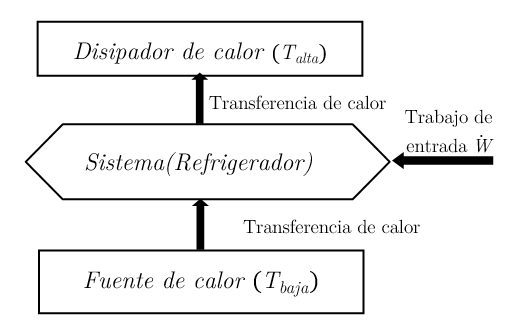
\includegraphics[width=0.7\linewidth]{figures/ciclo-termo}
	\caption{Ciclo termodinámico representando un refrigerador}
	\label{fig:ciclo-termo}
\end{figure}

\subsection{Tipos de cámaras frigoríficas usados en farmacéutica}



Basándose en el módulo III $"$Cadena de frío", del Curso de gerencia para el manejo efectivo del Programa Ampliado de Inmunización PAI, desarrollado por la Organización Panamericana de la Salud (OMPS) la cual es la Oficina Regional de Organización Mundial de la Salud en el año 2006. 

Se tiene que, para almacenar y conservar el medicamento del PAI se utilizan tres tipos de refrigeradores, 

\begin{enumerate}
	\item	Refrigerador por compresión eléctrica\\
	Se utiliza ampliamente para almacenar vacunas en establecimientos de salud con electricidad permanente (ver Figura \ref{fig:compresionelec})
	\begin{figure}[H]
		\centering
		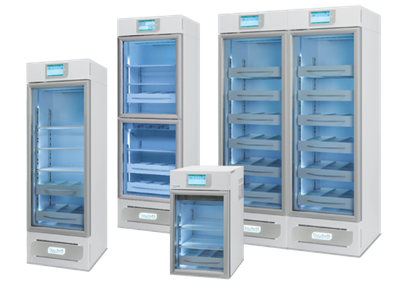
\includegraphics[width=0.6\linewidth]{figures/compresionelec}
		\caption{Refrigerador de laboratorio por compresión eléctrica.}
		Fuente: \cite{refrigeradores-2013}
		\label{fig:compresionelec}
	\end{figure}
	\item Refrigerador por absorción\\
	Los refrigeradores (que funcionan con propano o queroseno) son ideales para áreas sin electricidad o donde los recursos eléctricos son limitados (ver Figura \ref{fig:refexper} ).
	
	
	\begin{figure}[H]
		\centering
		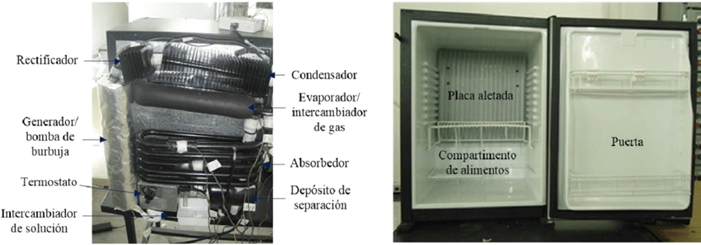
\includegraphics[width=0.6\linewidth]{figures/refexper}
		\caption{Refrigerador experimental difusión-absorción.}
		Fuente:  \cite{belamn-2015}
		\label{fig:refexper}
	\end{figure}
	
	\item Refrigerador fotovoltaico (energía solar)
	
	
	Los dispositivos solares son ideales para almacenar y conservar vacunas o medicamentos en áreas de difícil acceso, especialmente en áreas donde los recursos energéticos convencionales no están disponibles o son difíciles de obtener. Funciona con energía solar que se almacena en una batería para alimentar el refrigerador (ver Figura \ref{fig:refsolar}.
	
	
	\begin{figure}[H]
		\centering
		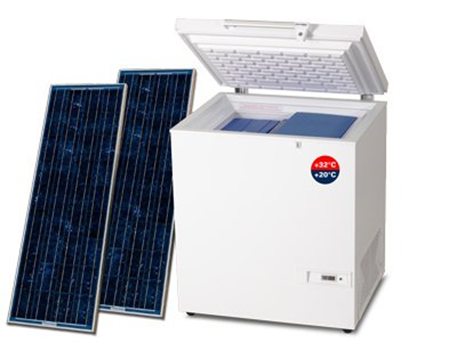
\includegraphics[width=0.6\linewidth]{figures/refsolar}
		\caption{Solarchill, el refrigerador Solar que salva vidas.}
		Fuente: \cite{ecoinventos-2022}
		\label{fig:refsolar}
	\end{figure}
	\item Equipos frigoríficos de pared de hielo (ice-lined refrigerators)\\
	
	Las unidades de enfriamiento de pared de hielo consisten en tubos o bolsas de enfriamiento llenos de líquido dispuestos alrededor de las paredes interiores del gabinete (Figura \ref{fig:reficeline}). Lo más importante es que tarda al menos 48 horas (+8 ºC) en calentarse en caso de corte de luz.
	
	\begin{figure}[H]
		\centering
		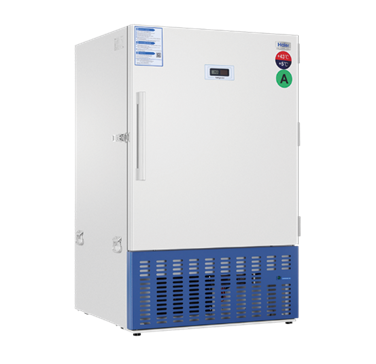
\includegraphics[width=0.6\linewidth]{figures/reficeline}
		\caption{Refrigerador con Revestimiento de Hielo Vertical.}
		Fuente: \cite{hunuo-technology}
		\label{fig:reficeline}
	\end{figure}
	
	
	\section{Contexto normativo}
	
	En un proyecto de diseño de ingeniería como el de la magnitud del presente (diseño de una cámara de refrigeración), es crucial que se conozcan las normas vigentes oficiales relacionadas con este tipo de proyectos. Esto se debe a que las normativas establecen estándares específicos que regulan diversos aspectos del diseño, construcción y operación de las cámaras de refrigeración.
	
	Por un lado las normas vigentes abordan aspectos relacionados con la seguridad, tanto para el personal que trabaja con la cámara como para los productos que se almacenan en ella. En tanto así, las normas pueden incluir requisitos para la instalación de sistemas de alarma, de ventilación y procedimientos de emergencia en caso de fallos en el equipo. Además deben incluir requisitos de temperatura específicos para diferentes tipos de productos, así como pautas para el monitoreo y registro de las condiciones del almacenamiento.
	
	Así mismo, las normas deben abordar aspectos relacionados con la eficiencia energética y el impacto ambiental de la cámara de refrigeración.
		
	\subsection{Normas Oficiales Mexicanas (NOM)}
	
		Las Normas Oficiales Mexicanas (NOM) son leyes técnicas de obligado cumplimiento emitidas por las autoridades competentes, cuyo objetivo es establecer las condiciones que deben cumplirse si un proceso o servicio representa un riesgo para la seguridad humana, o pone en peligro la salud humana. También contiene información sobre los términos y referencias para el cumplimiento y aplicación de estos términos \cite{salud-2022}.
		
		
		\begin{itemize}
			\item NOM-12-ENER-2019, Eficiencia energética de unidades condensadoras y evaporadoras para refrigeración. Límites, métodos de prueba y etiquetado.\\
			Esta Norma Oficial Mexicana establece los requisitos de eficiencia energética que deben cumplir las unidades condensadoras y evaporadoras, así como los métodos de prueba para verificar su cumplimiento, el etiquetado y el procedimiento para evaluar la conformidad de los productos.
			\begin{enumerate}
				\item Unidades condensadoras para refrigeración, que son fabricadas para su instalación al aire libre o en interiores con potencia frigorífica, mayor o igual que 746 W (2 547 BTU/h) y menor que 26 000 W (88 716 BTU/h) en media temperatura, y menor que 9 500 W (32 415 BTU/h) en baja temperatura.
				\item Unidades evaporadoras para refrigeración de bajo perfil que son destinadas para operar con un refrigerante y alimentados por expansión directa en condiciones húmedas y/o secas con capacidades nominales de enfriamiento, mayor o igual que 300 W (1 023 BTU/h) y menor que 40 000 W (136 482 BTU/h) en media temperatura, y menor que 13 000 W (44 397 BTU/h) en baja temperatura \cite{dof-2010}.
			\end{enumerate}
			
			\item  	NOM-008-SCFI-2002, Sistema General de Unidades de Medida. 
			
			Esta Norma Mexicana establece las definiciones, símbolos y reglas de notación para las unidades del Sistema Internacional de Unidades (SI) y otras unidades fuera de este sistema reconocidas por la CGPM, que en conjunto constituyen un sistema general de unidades de medida utilizadas en diversos campos en ciencia, tecnología, industria, educación y comercio \cite{dof-2010-nom008}.
			
			\item NOM-015-SSA2-2010, Para la prevención, tratamiento y control de la diabetes mellitus.
			
			Esta Norma Oficial Mexicana tiene por objeto establecer los procedimientos para la prevención, tratamiento, control de la diabetes y la prevención médica de sus complicaciones.
			También esta norma es de observancia obligatoria en el territorio nacional para los establecimientos y profesionales de la salud de los sectores público, social y privado que presten servicios de atención a la diabetes en el Sistema Nacional de Salud \cite{dof-2010-nom015}.
			
			\item NOM-028-STPS-2012, Sistema para la administración del trabajo-Seguridad en los procesos y equipos críticos que manejen sustancias químicas peligrosas.
			
			Establecer los elementos de un sistema de administración para organizar la seguridad en los procesos y equipos críticos que manejen sustancias químicas peligrosas, a fin de prevenir accidentes mayores y proteger de daños a las personas, a los centros de trabajo y a su entorno.
			
			\item	NOM-176-SSA1-1998, Validación de proveedores de fármacos y materias primas para la elaboración de medicamentos de uso humano.
			
			Esta Norma Oficial Mexicana establece los requisitos sanitarios que deben reunirse para la aprobación de proveedores de fármacos y materias primas de fabricación nacional o extranjera, utilizadas para la elaboración de medicamentos de uso humano.
			
			\item NOM-197-SSA1-2000, Que establece los requisitos mínimos de infraestructura y equipamiento de hospitales y consultorios de atención médica especializada.
			
			Esta Norma Oficial Mexicana tiene por objeto establecer los requisitos mínimos de infraestructura y de equipamiento para los hospitales y consultorios que presten atención médica especializad
			
					
		\end{itemize}	
\end{enumerate}

\subsection{Sociedad Americana de Ingenieros de Calefacción, Refrigeración y Aire Acondicionado (ASHRAE)}

La ASHRAE es la principal organización enfocada en el análisis técnico de las edificaciones desde hace más de 30 años. Formalmente se consolidó en el año 1984 y actualmente en 2024 cuenta con más de 57,000 miembros en todo el mundo. Estos integrantes conformados entre asociados y miembros se han centrado en la investigación, redacción de norma y publicación continua en sistemas de edificación, eficiencia energética, calidad del aire y sostenibilidad al interior de la industria \cite{ashrae-about}.


\begin{itemize}
	\item ANSI/ASHRAE Standard 34-2022, Designación y clasificación de seguridad de los refrigerantes.
	La Norma ASHRAE, crea una nomenclatura sencilla para referirse a los refrigerantes comunes, con el fin de no utilizar su nombre químico, fórmula o nombre comercial.
	 \begin{itemize}
	 
	 
	\item Los refrigerantes se numeran con una R-, seriada con un número propuesto por la ASHRAE.
	\item Una letra minúscula al final, si el refrigerante tiene un isómero (misma fórmula química, pero no de estructura química igual)
	\item Una letra mayúscula al final, si el refrigerante tiene los componentes puros iguales.
	\item Se añade “xxx” después de “R-” si el refrigerante es una mezcla con al menos otro refrigerante más. 
\end{itemize}
\end{itemize}


\subsection{Normas ISO}

La Organización Internacional de Normalización, es la organización internacional que gracias a todos sus expertos en todas las áreas, desde gestión de calidad a la inteligencia artificial se encargan de asegurarnos productos y servicios, seguros, fiables y de alta calidad.

\begin{itemize}
	\item ISO 5149:2014 – Sistemas de refrigeración mecánicos utilizados para enfriamiento y calefacción – Requisitos de seguridad.
	
	Especifica los requisitos relativos a la seguridad de las personas y los bienes para el diseño, fabricación, instalación y operación de sistemas de refrigeración, y pone el acento en reducir al mínimo las fugas de refrigerante a la atmósfera. 
	Es aplicable a todo tipo de sistemas de refrigeración en los que el refrigerante se evapora y se condensa en un circuito cerrado. 
	\item	ISO 817:2014 Refrigerantes – Designación y clasificación de seguridad
	
	Facilita un claro sistema de numeración y asignación de prefijos para la designación de la composición de los refrigerantes (p. ej., el prefijo CFC se utiliza para designar a los clorofluorocarbonos).
	Clasificaciones de seguridad de los refrigerantes según inflamabilidad y toxicidad.
	
	\item	ISO 11650:1999 Rendimiento de equipos para la recuperación y/o el reciclado de refrigerantes.
	
	Especificación de los aparatos de prueba, las pruebas de las mezclas de gases, los procedimientos de muestreo y las técnicas analíticas que se utilizarán para determinar el rendimiento de equipos para la recuperación y/o el reciclado de refrigerantes.
	
\end{itemize}

\section{Contexto geográfico}\label{sec:contex_geografico}
	Tener en cuenta el contexto geográfico en un proyecto de refrigeración es fundamental para adaptar el diseño y las especificaciones técnicas a las condiciones climáticas locales. Esto permite garantizar un rendimiento óptimo y eficiente de los sistemas de refrigeración, así como una mayor durabilidad y fiabilidad en diferentes entornos ambientales.
	
	
\subsection{Ubicación geográfica}

El proyecto será diseñado bajo condiciones específicas que residen en el interior de la Clínica número 40, la cual a sus vez es una Unidad Médica Familiar del IMSS, ésta se ubica en la avenida Hidalgo número 24 colonia entre Cerrada de Hidalgo y la Era en la colonia Santa Bárbara de la alcaldía Azcapotzalco Ciudad de México, CP 02230. En las figuras \ref{fig:mapsumf40} y \ref{fig:sateliteumf41} se aprecian la ubicación a través de Google Maps, (nivel de cuadra y calles) y en vista satelital (nivel Ciudad de México) respectivamente. 


\begin{figure}[H]
	\centering
	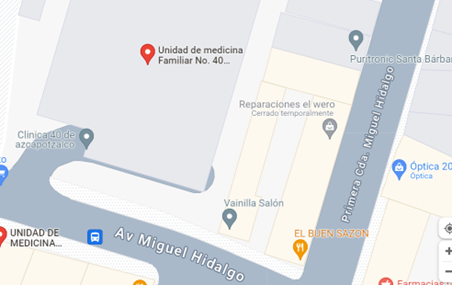
\includegraphics[width=0.6\linewidth]{figures/mapsumf40}
	\caption{Unidad Médica Familiar 40, Santa Bárbara Azcapotzalco Ciudad de México.}
	\label{fig:mapsumf40}
\end{figure}

\begin{figure}[H]
	\centering
	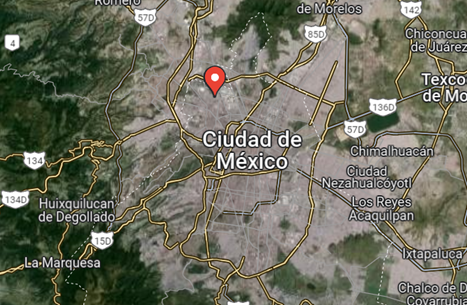
\includegraphics[width=0.6\linewidth]{figures/sateliteumf41}
	\caption{Vista satelital de la ubicación de la Unidad Médica Familiar 40 en Ciudad de México.}
	\label{fig:sateliteumf41}
\end{figure}

\subsection{Variables climáticas de la región}

Por propiedades espaciales para cuestiones climatológicas se hará uso a nivel de la Ciudad de México, puesto que las variaciones en la zona especificada del diseño son despreciables. 

En la Ciudad de México, de acuerdo a datos oficiales de INEGI, la mayor parte del territorio se tienen presencia de un clima Templado subhúmedo (87\%), en su parte restante se tiene un clima Seco y semiseco (7\%) y en Templado húmedo (6\%) (Ver figuras \ref{fig:climadf} y \ref{fig:calordf}).

Así mismo se sabe por estadísticas que la temperatura media anual es de 16°C, mientras que la más alta es mayor a los 25°C en los meses de marzo a mayo  y la menor está cercana a 5°C en enero. Las lluvias se presentan en verano, la precipitación total anual es variable: en la región seca es de 600 mm y en la parte templada húmeda (Ajusco) es de 1 200 mm anuales.
La zona urbana ocupa la mayor parte del territorio, pero hacia la parte sur y sureste se encuentran zonas agrícolas, principalmente de temporal, donde se cultiva maíz, frijol, avena y nopal entre otras, siendo importantes también las hortalizas y la floricultura. \cite{clima-df}.


\begin{figure}[H]
	\centering
	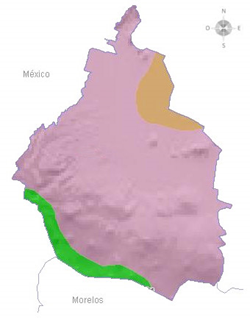
\includegraphics[width=0.6\linewidth]{figures/climadf}
	\caption{Condiciones climáticas de la Ciudad de México.}
	Fuente: \cite{clima-df}
	\label{fig:climadf}
\end{figure}

\begin{figure}[H]
	\centering
	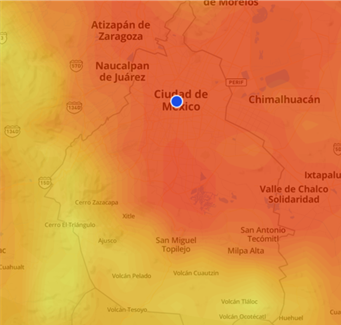
\includegraphics[width=0.6\linewidth]{figures/calordf}
	\caption{Mapa y radar del tiempo para Mexico city, DF (Weather Channel, 2024)}
	\label{fig:calordf}
\end{figure}


\section{Contexto del producto}


La diabetes mellitus (DM) forma un grupo de enfermedades crónico-degenerativa caracterizadas por hiperglucemia debido a defectos en la secreción y/o acción de la insulina. La hiperglucemia crónica se asocia con daños a largo plazo en varios órganos, especialmente los ojos, riñones,  los nervios, vasos sanguíneos y el corazón \cite{alfaro2002}.

La RAE\footnote{Real Academia Española}, (2023) y NCI\footnote{National Cancer Institute} , (s. f), coinciden que la insulina es aquella hormona desarrollada por los islotes de Langerhans en el páncreas (figura 2.10 (a)), que regula la cantidad de glucosa existente en la sangre.


\begin{figure}[H]
	\centering
	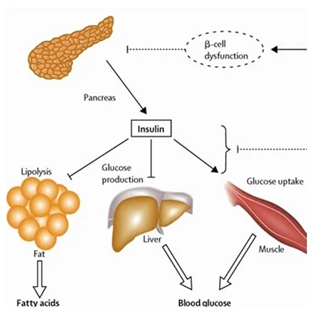
\includegraphics[width=0.36\linewidth]{figures/structureinsuline}	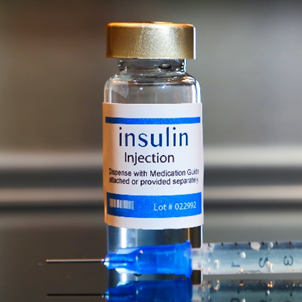
\includegraphics[width=0.36\linewidth]{figures/insulinbottle}\\
	(a) \hspace*{5cm} (b)
	\caption{a) Estructura de la insulina y su interacción con partes del cuerpo (Mandal, 2010) . (b) Frasco de insulina Inyectable comercial}
	Fuente: \cite{healthcentral2022}. 
	\label{fig:structureinsuline}
\end{figure}

Los productos de insulina alojados en frascos o cartuchos (figura 2.10 (b)) proporcionados por los fabricantes, tanto abiertos como cerrados, pueden mantenerse a temperatura ambiente, entre 59 °F y 86 °F, durante un máximo de 28 días sin que su eficacia se vea comprometida. Sin embargo, si la insulina ha sido diluida o extraída del envase original del fabricante, debe ser desechada dentro de un plazo de dos semanas \cite{research2017}.

Como ya se dijo antes, la insulina es una hormona polipeptídica, la cual estructuralmente en química está formada por 2 cadenas, una de 21 aminoácidos, la A y otra de 30 aminoácidos, la B, unidas por 2 enlaces disulfuro y existe un tercer enlace disulfuro dentro de la cadena A. \cite{gonzalez2017}.


\subsection{Almacenamiento de la insulina}

 
Los fabricantes de medicamentos ofrecen insulina en dos presentaciones básicas: viales y plumas.
 
Los requisitos generales de almacenamiento de la insulina enlistadas aquí siguen de una norma general que contemplan los distribuidores y consumidores a través de la cadena de suministro de la insulina (Ver figura \ref{fig:suministro}):

\begin{enumerate}
	 \item	La insulina congelada debe desecharse.
	\item	No utilice nunca la insulina después de la fecha de caducidad indicada en el vial, la pluma o el cartucho suministrado por el fabricante.
	\item	Nunca expongas la insulina al calor o la luz directa.
	\item Inspeccione la insulina antes de cada uso. No debe utilizarse ninguna insulina que presente grumos o partículas blancas sólidas.
\item La insulina debe ser transparente no debe tener ningún aspecto turbio.

	Formas de determinar si la insulina está en buenas condiciones, consulte la tabla 1 de alguno de los productos de insulina.
\begin{enumerate}
\item[i.]	La insulina sin abrir y sin usar debe almacenarse en un frigorífico a una temperatura de 2 a 8 °C.
\item[ii.]	La insulina abierta y en uso debe almacenarse a una temperatura ambiente inferior a 30°C, tal que la consuma en el menor tiempo posible.
\item[iii.]	Si recibe insulina por envío a domicilio, confirme siempre que la insulina se va a almacenar en condiciones adecuadas.
	\end{enumerate}
\end{enumerate}



\begin{figure}[H]
	\centering
	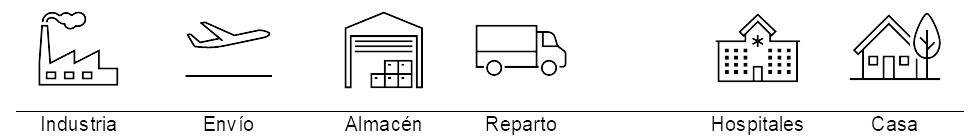
\includegraphics{figures/suministro}
	\caption{Cadena de suministro más común de la insulina Industria a Paciente}
	Fuente: Elaboración propia, basado de \cite{opsonu}.
	\label{fig:suministro}
\end{figure}



\begin{table}[H]
	\centering
	\caption{Calidad y caducidad específica aplicable a productos de insulina.}
	Fuente: \cite{jacob2023}.\\
	\begin{tabular}{@{}cccc@{}}
		\toprule
		\multicolumn{1}{l}{\textbf{Producto}} & \multicolumn{1}{l}{\textbf{Sin abrir}} & \textbf{\begin{tabular}[c]{@{}c@{}}Abierto \\ (Temperatura ambiente $T_{amb}$ )\end{tabular}} & \multicolumn{1}{l}{\textbf{Sello dañado}} \\ \midrule
		\underline{\textbf{Viales:}}                & \multicolumn{3}{l}{}                                                                                                                                                    \\
		Fiasp®                                & Fecha de caducidad                     & 28 días                                                                            & 28 días                                   \\
		Humulin R                             & Fecha de caducidad                     & 31 días                                                                            & 31 días                                   \\
		Novolin                               & Fecha de caducidad                     & 42 días                                                                            & 42 días ($T_{amb}$)            \\
		\underline{\textbf{Bolígrafos:}}   & \multicolumn{3}{l}{} \\
		Fiasp®                                & Fecha de caducidad                     & 28 días                                                                            & 28 días                                   \\
		Humulin N Pen                         & Fecha de caducidad                     & 14 días                                                                            & 14 días                                   \\
		Lyuumjev®                             & Fecha de caducidad                     & 28 días                                                                            & No refrigerar                             \\ \bottomrule
	\end{tabular}
	\label{tabla:caducidades}
\end{table}


\textbf{Nota}: La tabla \ref{tabla:caducidades} es una  referencia de investigación no está destinada a usarse como herramienta para hacer prescribir insulina\footnote{La insulina pierde eficacia al exponer a temperaturas elevadas, lo que  puede con llevar a la disminución del control de glucosa en la sangre, no se debe exponer insulina a más de 30°C}.









	 
